\documentclass[11pt]{book}
\usepackage{amsmath,amssymb,graphicx}
\usepackage{../setspace}
\usepackage{color}
\addtolength{\textwidth}{1.5in}
\addtolength{\hoffset}{-1in}
\addtolength{\textheight}{1.5in}
\addtolength{\voffset}{-1in}
\usepackage{/usr/share/R/share/texmf/Sweave}

\title{STAT3401 Multivariate Lab Workbook}
\author{Paul Hewson}
\begin{document}
\setlength{\parindent}{0pt}
\setlength{\parskip}{12pt}
\sffamily



\maketitle


\chapter*{Introduction}

Hello and welcome to the multivariate statistics part of STAT3401.   One word of caution about these notes.   The first column of the notes will have either a $>$ or a $+$ symbol denoting the R prompt or the ``R command carrying over an additional line''.   You don't need to type that in.  

I might put some of the longer R functions in the portal, to save a little typing.   Nevertheless, you do need to \emph{understand} what you are doing.


\chapter{Week 1: EDA}

Monday 28th September



\section{Multivariate eda}

Graphical exploration of data is essential.   There are a wide range of techniques for use with multivariate data, this week we examine some of the more common ones.   The aim of this week is to introduce you to some of these techniques, and provide pointers for more advanced ones.   You should save the code you use to generate these graphs in a short script file for future reference!


\section{A correlation paradox}

Here's the correlation paradox we referred to.   Can you explain what's going on here?

\begin{Schunk}
\begin{Sinput}
> u <- rnorm(100)
> v <- rnorm(100)
> w <- rnorm(100)
> x <- u + v
> y <- u + w
> z <- v - w
> X <- cbind(x, y, z)
> cor(X)
> pairs(X)
\end{Sinput}
\end{Schunk}


\section{Key eda techniques}

First, we need to load some data and obtain the most important summary statistics.   We will load data on USArrests as well as irises.   As you go through the lab, if appropriate do try to produce graphs for the other dataset.

\begin{Schunk}
\begin{Sinput}
> data(USArrests)
> `?`(USArrests)
> cov(USArrests)
> cor(USArrests)
> colMeans(USArrests)
> data(iris)
> `?`(iris)
\end{Sinput}
\end{Schunk}

There are then a few ways of producing the ``standard'' pairwise scatterplots.

\begin{Schunk}
\begin{Sinput}
> pairs(USArrests)
> library(lattice)
> splom(USArrests)
\end{Sinput}
\end{Schunk}


As well as examining the relationships between variables, we may be interested in the relationship between individuals.

\begin{Schunk}
\begin{Sinput}
> heatmap(as.matrix(USArrests))
> stars(USArrests, col.segments = c("red", "green", "blue", "pink"), 
+     draw.segments = TRUE, full = FALSE)
> require(MASS)
> parcoord(iris[, -5], col = as.numeric(iris[, 5]))
> source("andrews.R")
> andrews.curves(iris[, -5], cls = iris[, 5])
\end{Sinput}
\end{Schunk}

You can see for example that \texttt{parcoord} and \texttt{andrews.curves} take a data matrix as the first argument (in this case we specify the first four columns of the iris data), and a grouping factor as the second argument (with slightly different syntax).


\section{Interactive Graphics}

You've been given a short piece of code in the portal which helps draw 3d scatterplots on the \texttt{rgl} device.   If you put this code in your working directory and ``source'' it, you should be able to create a simple dynamic 3d scatterplot.   Check out \texttt{?rgl} if you want any help on the rgl device, in particular to see how you might go about saving an image!

%<<rgl, fig = FALSE, echo = TRUE, results = hide>>=

\begin{verbatim}
source("rglellipsoid.R")
scatter3d(iris$Sepal.Length, iris$Sepal.Width, iris$Petal.Width,
           ellipsoid=TRUE, surface=FALSE,
           groups=as.factor(iris$Species))
\end{verbatim}
%@ 


\section{Simulating multivariate normal data and linear combinations}

First, load the \texttt{MASS} library which contains a function \texttt{mvrnorm} which simulates multivariate normal data.   The first argument to \texttt{mvrnorm} is $n$, the number of variate rows to generate, the second argument is the mean vector to use.   Here you see that we want to generate three observations, each with mean zero.   Finally, we need to specify the covariance matrix, we have done this on the previous line and stored the results in \texttt{covmat}.


\begin{Schunk}
\begin{Sinput}
> library(MASS)
> covmat <- matrix(c(1, 0.7, 0.7, 0.7, 1, 0.7, 0.7, 0.7, 1), 3, 
+     3)
> X <- mvrnorm(1000, c(0, 0, 0), covmat)
\end{Sinput}
\end{Schunk}


Having simulated some data (stored in the matrix \texttt{X}), we are going to check the univariate normality of each margin.   The code below produces histograms and plots for the second column, you should check all three!

\begin{Schunk}
\begin{Sinput}
> hist(X[, 2])
> qqnorm(X[, 2])
> qqline(X[, 2], col = "red")
\end{Sinput}
\end{Schunk}
\includegraphics{week1eda-uvnorm}

Finally, to start thinking about linear combinations, try generating a few linear combinations e.g. $z_{i} = 2x_{i1}+0.2x_{i2}+0.15x_{i3}$ for all $i = 1, \ldots, n$.

\begin{Schunk}
\begin{Sinput}
> Z <- 2 * X[, 1] + 0.2 * X[, 2] + 0.15 * X[, 3]
> hist(Z)
\end{Sinput}
\end{Schunk}

Try different values for the coefficients (i.e replace $2, 0.2 and 0.15$ with other values) and see whether $\boldsymbol{z}$ can be considered to be univariate normal.


\section{On your own}

Load the following libraries, and check out the following functions and data files:   

\begin{itemize}
\item Libraries: \texttt{library(gclus)}, \texttt{library(Flury)}
\item Functions: \texttt{?cpairs}, \texttt{?cparcoord} 
\item Data: \texttt{data(wines)}, \texttt{data(turtles)} and \texttt{data(flea.beetles)} (in other words, load the data and look at the helpfiles in the same way you check the helpfile for a function)
\end{itemize}



Do also check out the correlation demo:

\begin{verbatim}
library(TeachingDemos)
run.cor.examp()
\end{verbatim}






\section{Summary of week1}

\fbox{\parbox[c]{0.9\textwidth}{\color{blue}
\begin{itemize}
\item You should have answered the correlation paradox (although we will either discuss it in the lab or in the lecture in week 2)
\item You have started collecting a library of scripts that let you carry out a multivariate e.d.a. - for example you have a few lines of R that let you create star plot, with suitable legends and labels.   Save these carefully as we will assume from now on that given a set of data, you can quickly and efficiently conduct an exploratory data analysis
  \end{itemize}

}}


\chapter{Week 2: Matrices}

Monday 5th October



\section{Computer exercises for the lab}

This week is a good time for
\begin{itemize}
\item[(a)] making sure you are comfortable with the mathematics behind matrices as well as:
\item[(b)] making sure you are comfortable with the matrix operators in R.   
\item[(c)]  Check that you are very very sure you can subscript R matrices, i.e. use things such as \text{[,1]} to select column 1, \text{[,-1]} to select everything \emph{except} column 1, and \text{[,2:3]} to select columns 2 and 3.
\end{itemize}

Although we will use in built multivariate analysis functions in R, you should consider checking you understand the techniques by using R as a matrix calculator.
  
\begin{enumerate}

\item Find (where possible) the determinants and the inverse of the following matrices:

$C_{1} = \left[ \begin {array}{cc} 4& 4\\\noalign{\medskip} 4& 4\end {array} \right]$, $C_{2} = \left[ \begin {array}{cc} 4& 4.001\\\noalign{\medskip} 4.001& 4.002\end {array} \right]$ and $C_{3} = \left[ \begin {array}{cc} 4& 4.001\\\noalign{\medskip} 4.001& 4.002001\end {array} \right] $

Very briefly comment on the magnitude of the difference between $C_{2}^{-1}$ and  $C_{3}^{-1}$ given the only difference between $C_{2}$ and $C_{2}$ amounts to a difference of $0.000001$ in the bottom right position.

\begin{Schunk}
\begin{Sinput}
> A <- matrix(c(4, 4, 4, 4), 2, 2)
> A
> det(A)
> try(solve(A))
> B <- matrix(c(4, 4.001, 4.001, 4.002), 2, 2)
> B
> det(B)
> solve(B)
> C <- matrix(c(4, 4.001, 4.001, 4.002001), 2, 2)
> C
> det(C)
> solve(C)
\end{Sinput}
\end{Schunk}


\begin{itemize}
  \item What's going on here?
\end{itemize}

\textit{Note that A is singular, the determinant is zero and it can't be inverted.   Also note that the inverses of B and C are very very different - but this is something of a pathological example}


\item Matrix partitioning.   Consider Sterling's financial data held in the R object LifeCycleSavings (see \verb+?LifeCycleSavings+).   To make life a little easier, reorder the columns using \texttt{X <- LifeCycleSavings[,c(2,3,1,4,5)]}.
  

\begin{itemize}
\item Find the correlation matrix of \texttt{X} (longhand, using the centering matrix), call this matrix \texttt{R}


\begin{Schunk}
\begin{Sinput}
> data(LifeCycleSavings)
> X <- LifeCycleSavings[, c(2, 3, 1, 4, 5)]
> R <- cor(X)
> R
\end{Sinput}
\end{Schunk}


\item Partition \textit{R = cov(X)} following the scheme below such that $\boldsymbol{R_{11}}$ is a $2 \times 2$ matrix containing the covariance of \texttt{pop15} and \texttt{pop75}, and $\boldsymbol{R_{22}}$ contains the covariance of \texttt{sr}, \texttt{dpi} and \texttt{ddpi}

\begin{displaymath}
\boldsymbol{R} = \left( \begin{array}{l|l} \boldsymbol{R_{11}} & \boldsymbol{R_{12}} \\ \hline    \boldsymbol{R_{21}} & \boldsymbol{R_{22}} \end{array} \right) 
\end{displaymath}

You should find for example that  $\boldsymbol{R_{11}}$ is given by:
 % latex table generated in R 2.3.1 by xtable 1.3-2 package
% Wed Nov 15 22:15:30 2006
\begin{table}[ht]
\begin{center}
\begin{tabular}{rrr}
\hline
 & pop15 & pop75 \\
\hline
pop15 & 83.75 & $-$10.73 \\
pop75 & $-$10.73 & 1.67 \\
\hline
\end{tabular}
\end{center}
\end{table}

\begin{Schunk}
\begin{Sinput}
> R11 <- R[1:2, 1:2]
> R12 <- R[1:2, 3:5]
> R21 <- R[3:5, 1:2]
> R22 <- R[3:5, 3:5]
> R11
> R22
> R21
> R12
> t(R21)
\end{Sinput}
\end{Schunk}


\item Find the matrix $\boldsymbol{A}$, where:

\begin{displaymath}
\boldsymbol{A} = \boldsymbol{R_{22}^{-1}R_{21}R_{11}^{-1}R_{12}}
\end{displaymath}



\begin{Schunk}
\begin{Sinput}
> A <- solve(R22) %*% R21 %*% solve(R11) %*% R12
\end{Sinput}
\end{Schunk}


%\begin{itemize}

\item Are $\boldsymbol{A}$ and $\boldsymbol{B}$ symmetric?   What is the difference between symmetric and asymmetric matrices in terms of their eigenvalues and eigenvectors?\\
\textit{Note that they are both asymmetric matrices, it just so happens for these particular matrices that the eigenvalues are positive and the eigenvectors are real.   This isn't always the case for asymmetric matrices!}

\item Find the eigenvalues and eigenvectors of $\boldsymbol{A}$ and $\boldsymbol{B}$ then find the square roots of the eigenvalues.   


\begin{Schunk}
\begin{Sinput}
> eigen(B)
> sqrt(eigen(A)$values)
> sqrt(eigen(B)$values)
\end{Sinput}
\end{Schunk}


\item Do you notice any similarities between the first two eigenvalues from either matrix?\\
\textit{Note that the square roots of the eigen values are identical.}
\end{itemize}

\item Revisit the \texttt{wines} data in the \texttt{Flury} package.   Consider only Y1, Y5, Y6, Y8 and Y9, use matrix algebra to find the means, correlation and covariance of these data.   Compare the eigenvalues and eigenvectors, and the determinants and inverse you get from the covariance matrix and the correlation matrix.\\


  
  
\end{enumerate} 


\section{Summary of week 2}

\fbox{\parbox[c]{0.9\textwidth}{\color{blue}
    
\begin{itemize}
\item We have revised, and are comfortable with matrix multiplication, matrix inverse, (normalised) eigenvalues and eigenvectors.  We can center and scale matrices.  We can do this by hand and in R.
\item We are also comfortable using R as a matrix calculator if and when we wish.
\end{itemize}
}}


\chapter{Week 3: Distance measures}

Monday 12th October


\section{Mahalanobis distance and multivariate normality}

\begin{Schunk}
\begin{Sinput}
> USA.mah.dist <- mahalanobis(USArrests, center = mean(USArrests), 
+     cov = var(USArrests))
> hist(USA.mah.dist, freq = FALSE)
> curve(dchisq(x, df = 4), add = TRUE, col = "red")
\end{Sinput}
\end{Schunk}

or consider $qq$ plots:

\begin{Schunk}
\begin{Sinput}
> n <- 50
> p <- 4
> qqplot(USA.mah.dist, qchisq(ppoints(n), p))
\end{Sinput}
\end{Schunk}


\begin{itemize}
\item Do you think that the USArrests data can be considered to be multivariate normal.   If so, repeat this with some other data, such as the simulated multivariate normal data you generated in week 1, or any other data we have met (e.g. iris data).
\item For any data you consider, compare your findings on multivariate normality with what you find when examining univariate normality of either the margins or the linear combinations
\end{itemize}

More advanced work: there are some who think that a beta distribution should be used.   There is a function \texttt{qqbetaM} in a file in the portal.   Copy this into your workspace, \texttt{source} the function and see whether you think it makes a difference.     

\begin{Schunk}
\begin{Sinput}
> source("qqbetaM.R")
> qqbetaM(USA.mah.dist, 4)
\end{Sinput}
\end{Schunk}

Compare the qqplots you obtain from this function with qqplots from the $\chi^{2}$ based quantiles.   Do you have any data where your impression of normality may be altered by a change in the comparison?   From your reading material, when might it matter whether you use a beta distribution or a $\chi^{2}$?

\section{Gower's distance}

This is quite an important exercise!   Make sure you are happy calculating Gower's distance.  Use the \texttt{class08.csv} data in the portal, and calculate the distance between a few individuals by hand.   Then use \texttt{daisy} in \texttt{library(cluster)} to calcuate it in R (it's a slightly fiddly function to use). 



\section{Summary}
\fbox{\parbox[c]{0.9\textwidth}{\color{blue}
By the end of week 3 we should be able to:

\begin{itemize}
\item appreciate the role of the Mahalanobis distance in relation to the multivariate normal distribution
\item be able to calculate a range of distance measures for continuous, categorical, binary and mixed data.   We know the R functions for doing these calculations, but can also carry out examples of the calculation by hand
\end{itemize}
}}


\chapter{Week 4: Cluster analysis}

Monday 19th October



\section{Preliminaries and exploratory data analysis}

We start off by loading a useful support library, the \texttt{cluster} library.   We need to load the \texttt{flexclust} library to get hold of some interesting data.   Make that data available (the \texttt{milk} data) and start doing an exploratory data analysis.   The suggested code here includes star plots (quite interesting here) and faces (not very useful).   You may also consider parallel co-ordinates plots and scatterplots, but we will come back to them later.

\begin{Schunk}
\begin{Sinput}
> library(cluster)
> library(flexclust)
> library(MASS)
> library(TeachingDemos)
> data(milk)
> stars(milk, full = FALSE, draw.segments = TRUE, key.loc = c(10, 
+     0.4), main = "Milk data")
> faces(milk, fill = TRUE, ncol = 4, scale = TRUE, nrow = 7)
\end{Sinput}
\end{Schunk}


\section{Calculating distances and performing hierarchical clustering}

The first piece of clustering will demonstrate the defaults, i.e. euclidean distance and complete linkage.   A good habit is to create a distance object, then create a \texttt{hclust} object and then extract whatever information we need from that \texttt{hclust} object.   For example, \texttt{plot()} will produce a dendrogram and \texttt{cutree()}, given an argument for \texttt{k} will ``cut'' the tree at the given number of clusters (you can also cut based on height if you prefer)

\begin{Schunk}
\begin{Sinput}
> milk.dist <- dist(milk)
> milk.hclust <- hclust(milk.dist)
> plot(milk.hclust)
> milk.cut <- cutree(milk.hclust, 3)
\end{Sinput}
\end{Schunk}


It is of interest investigating the stability of your cluster solution to different choices of distance measure, for example using the Manhattan distance:

\begin{Schunk}
\begin{Sinput}
> milk.dist.man <- dist(milk, method = "manhattan")
> milk.hclust.man <- hclust(milk.dist.man)
> plot(milk.hclust.man)
> milk.cut.man <- cutree(milk.hclust.man, 3)
> xtabs(~milk.cut + milk.cut.man)
\end{Sinput}
\end{Schunk}

or the Minkowski, with $\lambda=5$ (R calls this \texttt{p})

\begin{Schunk}
\begin{Sinput}
> milk.dist.min5 <- dist(milk, method = "minkowski", p = 5)
> milk.hclust.min5 <- hclust(milk.dist.min5)
> plot(milk.hclust.min5)
> milk.cut.min5 <- cutree(milk.hclust.min5, 3)
> xtabs(~milk.cut + milk.cut.min5)
\end{Sinput}
\end{Schunk}


Also, one may wish to consider different clustering strategies, in this case we consider Ward's method (based on the Euclidean distance):

\begin{Schunk}
\begin{Sinput}
> milk.hclust.ward <- hclust(milk.dist, method = "ward")
> plot(milk.hclust.ward)
> milk.cut.ward <- cutree(milk.hclust.ward, 3)
> xtabs(~milk.cut + milk.cut.ward)
\end{Sinput}
\end{Schunk}


You should actually find for these data, whatever you do yields quite a stable three cluster ``solution''.


\section{Visualising the solution in terms of the data}

We can use some standard exploratory data analysis techniques, only in this case it is possible to ``label'' the rows in terms of the cluster membership we have proposed:

\begin{Schunk}
\begin{Sinput}
> parcoord(milk, col = milk.cut, lty = milk.cut, main = "milk data, four group clustering")
> pairs(milk, lower.panel = function(x, y) {
+     points(x, y, pch = milk.cut, col = milk.cut)
+ }, main = "Scatterplot for milk data")
\end{Sinput}
\end{Schunk}

\section{k-means clustering}

k-means clustering assumes we have some idea of $k$ before we start.   In this example, we seem to be quite sure that $k=3$, that won't necessarily be the case with other problems.   The \texttt{kmeans} object contains other information about the solution, such as the centroids, but the cluster assignments are easily extracted and compared with the solutions we found earlier.

\begin{Schunk}
\begin{Sinput}
> milk.kmeans <- kmeans(milk, centers = 3)
> milk.kmeans$cluster
> xtabs(~milk.cut + milk.kmeans$cluster)
\end{Sinput}
\end{Schunk}

Do note that k-means clustering is applied to the \emph{data} and \emph{not} to the distance matrix!!!!!!

\section{Measures of fit}

This is a massive area.   We consider just one possibility amongst many based on the cophenetic distance, a measure of the distance between the level at which two points are merged.   Measuring the correlation between this distance and the original distance matrix tells us something about how well a given dendrogram represents a given distance matrix.

\begin{Schunk}
\begin{Sinput}
> d.retained <- cophenetic(milk.hclust)
> cor(milk.dist, d.retained)
\end{Sinput}
\end{Schunk}

(Too) many more possibilities are given in \texttt{cluster.stats()} in \texttt{library(fpc)}.   One of the more common ones is the Rand statistic, which can be used to compare two cluster solutions.   Again, we supply the original distance matrix, and then the cluster solution we have chosen and an alternative.   You should find with the milk data that the Rand statistic = 1, as these solutions agree perfectly.  The helpfile for this function gives you references to the literature if you want to know what all the other statsitics are measuring.

\begin{Schunk}
\begin{Sinput}
> library(fpc)
> cluster.stats(milk.dist, milk.cut, alt = milk.cut.man)
\end{Sinput}
\end{Schunk}



\section{Summary}


\fbox{\parbox[c]{0.9\textwidth}{\color{blue}
This week, we should have:

\begin{itemize}
\item Quickly carried out an e.d.a. using scripts saved from week 1 in order to look for similar subgroups within a dataset
\item Carried out cluster analysis using a variety of hierarchical schemes as well as k-means clustering
\item be able to describe the difference between hierarchical and k-means clustering; and to demonstrate this understanding by working simple examples by hand
\item be able to interpret the results of a cluster analysis; and  explain whether a particular hierarchical cluster analysis can be considered a ``good'' fit
\end{itemize}
}}


\chapter{Week 5: Principal components analysis}

Monday 26th October

\input{week5pca}

%\chapter{Week 6: Self Study (Canonical Correlation)}

%\chapter{Canonical Correlation}
\label{cancor}

\section{Canonical variates}
\label{canvar}

\section{Interpretation}
\label{canint}
%%%%%\chapter{Canonical Correlation}

In canonical correlation, we are interested in the relationship between two sets of variables.   We do this by creating linear combinations $\boldsymbol{U} = \boldsymbol{a_{1} x_{1}} + \boldsymbol{a_{2} x_{2}} + \cdots + \boldsymbol{a_{p} x_{p}}$ and  $\boldsymbol{V} = \boldsymbol{b_{1} y_{1}} + \boldsymbol{b_{2} y_{2}} + \cdots + \boldsymbol{b_{q} y_{q}}$ such that the correlation between $\boldsymbol{U}$ and $\boldsymbol{V}$ is as high as possible.


To do this, we need to work out the correlation matrix, and partition it:


\begin{displaymath}
\begin{array}{ccccccc} & x_{1} & \ldots & \_{p} & y_{1} & \ldots & y_{q} \end{array}
\end{displaymath}
\begin{displaymath}
\begin{array}{c} x_{1} \\ \vdots \\ x_{p} \\y_{1} \\ \vdots \\y_{3}\end{array}
\left( \begin{array}{ccc|ccc} &&&&&\\&A_{p \times p}& &C_{p \times q}&\\&&&&&\\
\hline
&&&&&\\&C_{q \times p}& &B_{q \times q}&\\&&&&&\\ \end{array} \right)
\end{displaymath}

Having done this, we calculate the matrix:

\begin{displaymath}
\boldsymbol{B^{-1}C^{T}A^{-1}C}
\end{displaymath}

and find the associated eigenvalues (in descending order)  $\lambda_{1} > \lambda_{2} > \ldots > \lambda_{r}$.   The corresponding eigenvectors $\boldsymbol{b_{1}}, \boldsymbol{b_{2}}, \ldots, \boldsymbol{b_{r}}$ give the coefficients of the Y variables.

So: 

\begin{displaymath}
\boldsymbol{v_{i}} = \boldsymbol{b_{i}^{T}} \boldsymbol{Y}
\end{displaymath}

where $\boldsymbol{b_{i}} = \left(\begin{array}{c} b_{i1} \\ \vdots \\ b_{iq} \end{array} \right)$ and $\boldsymbol{Y} = \left(\begin{array}{c} \boldsymbol{y_{1}} \\ \vdots \\ \boldsymbol{y_{q}} \end{array} \right)$, or in longhand:

\begin{displaymath}
\boldsymbol{v_{i}} = b_{i1} \boldsymbol{y_{1}} + \cdots + b_{iq} \boldsymbol{y_{q}}
\end{displaymath}

Having calculated these, it is possible to solve the coefficients for the X variables:

$a_{1} = \boldsymbol{A^{-1} C b_{1}}, a_{2} = \boldsymbol{A^{-1} C b_{2}}, \ldots,  a_{r} = \boldsymbol{A^{-1} C b_{r}}$,

f
\begin{displaymath}
\boldsymbol{u_{i}} = \boldsymbol{a_{i}^{T}} \boldsymbol{X}
\end{displaymath}


where $\boldsymbol{a_{i}} = \left(\begin{array}{c} a_{i1} \\ \vdots \\ a_{iq} \end{array} \right)$ and $\boldsymbol{X} = \left(\begin{array}{c} \boldsymbol{x_{1}} \\ \vdots \\ \boldsymbol{x_{r}} \end{array} \right)$, or in longhand:

\begin{displaymath}
\boldsymbol{u_{i}} = a_{i1} \boldsymbol{x_{1}} + \ldots + a_{ir} \boldsymbol{x_{r}}
\end{displaymath}

And one really cute result is that $\left[corr(\boldsymbol{u_{i}}, \boldsymbol{v_{i}})\right]^{2} = \lambda_{i}$.

\section{Computer example}

Franco Modigliani proposed a life cycle savings model, the savings ratio (aggregate personal saving divided by disposable income) is explained by per-capita disposable income, the percentage rate of change in per-capita disposable income, and two demographic variables: the percentage of population less than 15 years old and the percentage of the population over 75 years old. 

However, we are interested here in the relationship between the two demographic variables (percent of population under 15, percent of population over 75) and the three financial variables (personal savings, per-capita disposal income, growth rate of dpi).   The first stage of any such analysis would be a visual inspection.


\begin{verbatim}
pairs(LifeCycleSavings, pch = 16)
\end{verbatim}

\begin{figure}
\begin{center}
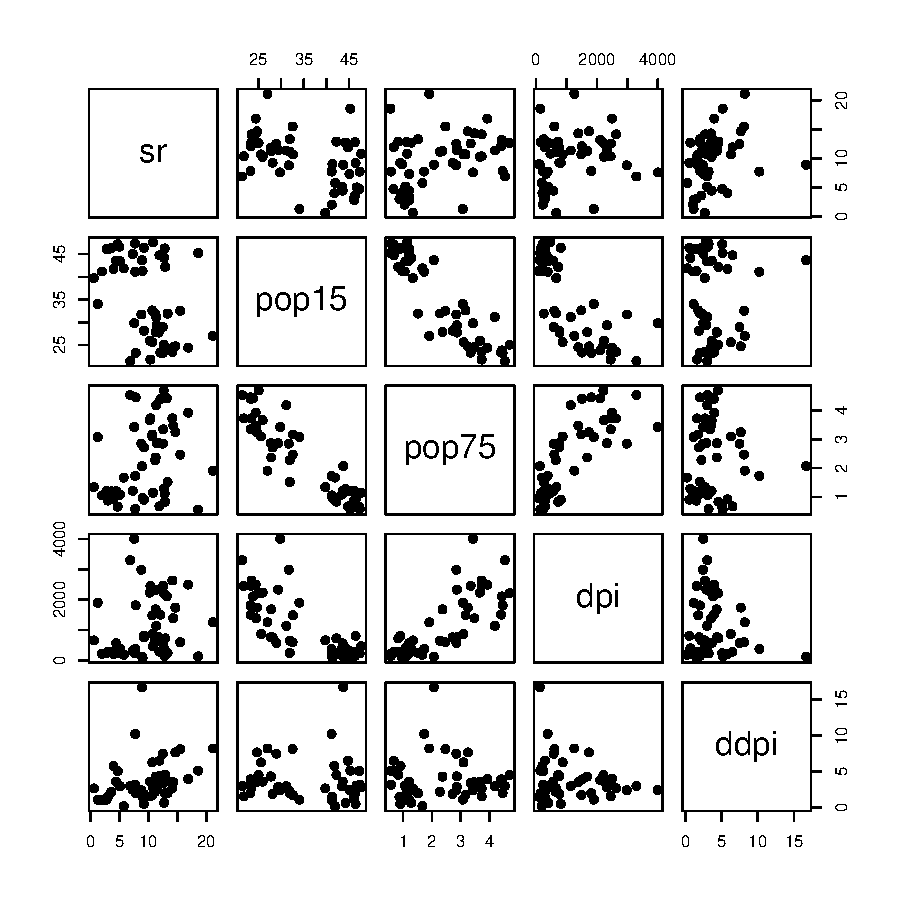
\includegraphics[width = 0.6\textwidth]{images/cancor}
\caption{Pairwise scatterplots of Life Cycle Savings data}
\end{center}
\end{figure}

And it is worth examining the correlation matrix:

\singlespacing
\begin{verbatim}
> cor(LifeCycleSavings)
              sr       pop15       pop75        dpi        ddpi
sr     1.0000000 -0.45553809  0.31652112  0.2203589  0.30478716
pop15 -0.4555381  1.00000000 -0.90847871 -0.7561881 -0.04782569
pop75  0.3165211 -0.90847871  1.00000000  0.7869995  0.02532138
dpi    0.2203589 -0.75618810  0.78699951  1.0000000 -0.12948552
ddpi   0.3047872 -0.04782569  0.02532138 -0.1294855  1.00000000
\end{verbatim}
\onehalfspacing

It appears that the \textbf{X} variables are correlated.   This is less so for \textbf{Y} variables, and even less so for \textbf{X,Y} inter-correlations.

You need to be sure that the variables are \emph{scaled} before carrying out a canonical correlation analysis.   

\singlespacing
\begin{verbatim}
LifeCycleSavingsS <- scale(LifeCycleSavings)
pop <- LifeCycleSavingsS[, 2:3] ## The X matrix
oec <- LifeCycleSavingsS[, -(2:3)] ## the Y matrix
\end{verbatim}
\onehalfspacing

Having created an \textbf{X} matrix and a \textbf{Y} matrix, we now want to find linear combinations of \textbf{X} which have maximum correlation with \textbf{Y}.

\singlespacing
\begin{verbatim}
> cancor(pop, oec)
$cor
[1] 0.8247966 0.3652762

$xcoef
             [,1]       [,2]
pop15 -0.08338007 -0.3314944
pop75  0.06279282 -0.3360027

$ycoef
           [,1]        [,2]         [,3]
sr   0.03795363  0.14955310 -0.023106040
dpi  0.12954600 -0.07518943  0.004502216
ddpi 0.01196908 -0.03520728  0.148898175

$xcenter
        pop15         pop75 
-4.662937e-16  2.753353e-16 

$ycenter
          sr          dpi         ddpi 
1.421085e-16 6.661338e-17 4.440892e-16 
\end{verbatim}
\onehalfspacing

This indicates one canonical correlate with a correlation of 0.8247966 between $z_{\boldsymbol{X}1}$ and $z_{\boldsymbol{Y}1}$

\begin{eqnarray}
z_{\boldsymbol{X}1} =  -0.08338007  x_{pop15} + 0.06279282 x_{pop75}\\
z_{\boldsymbol{Y}1} = 0.03795363 y_{sr} + 0.12954600 y_{dpi} +  0.01196908 y_{ddpi}
\end{eqnarray}

If we extract the coefficients as vectors (this time we have created \texttt{LCS.cancor} as an object; also we have used \texttt{as.numeric(\ldots)} to extract the coefficients in a form suitable for matrix multiplication).

\singlespacing
\begin{verbatim}
> LCS.cancor <- cancor(pop, oec)
> ycoef <- as.numeric(LCS.cancor$ycoef[,1])
> xcoef <- as.numeric(LCS.cancor$xcoef[,1])
> v1 <-  oec %*% ycoef ## remember oec and pop are scaled
> u1 <-  pop %*% xcoef
> plot(v1, u1)
> identify(v1, u1, row.names(LifeCycleSavings))
\end{verbatim}
\onehalfspacing


\subsection{Interpreting the canonical variables}

There is some ``controversy'' about the best way of interpreting the canonical variables.   You have two possibilities:

\begin{itemize}
\item Interpret the coefficients in a similar way to that used in principal components (problems with collinear variables)
\item Calculate the correlation between the canonical and the original variables (doesn't tell you anything about joint contributions)
\end{itemize}

%Consider:

%$\rho_{\hat{U},\boldsymbol{x}}$ = matrix of correlations between $\hat{U}$ and $\boldsymbol{x}$\\ 
%$\rho_{\hat{V},\boldsymbol{y}}$ = matrix of correlations between $\hat{V}$ and $\boldsymbol{y}$ \\
%$\rho_{\hat{U},\boldsymbol{y}}$ = matrix of correlations between $\hat{U}$ and $\boldsymbol{y}$ \\
%$\rho_{\hat{V},\boldsymbol{x}}$ = matrix of correlations between $\hat{V}$ and $\boldsymbol{x}$\\ 

%Which can be obtained fairly simply as:

%\begin{eqnarray*}
%\rho_{\hat{U},\boldsymbol{x}} = a \Sigma_{11}



\subsection{Hypothesis testing}

As with Principal Components, a certain amount of hypothesis testing is possible.   The distributional properties of canonical variables is far wilder than principal components - none of the recommended books discuss it.   However, the tests can be described.   For example, if we wanted to test whether there was any relationship between our two sets of variables:

\begin{displaymath}
H_{0}; \boldsymbol{\Sigma}_{12} = \boldsymbol{0}
\end{displaymath}

The Likelihood ratio test leads us to:

\begin{displaymath}
\Lambda^{\frac{2}{n}} = |\boldsymbol{I} - \boldsymbol{S_{22}^{-1}}\boldsymbol{S_{21}}\boldsymbol{S_{11}^{-1}}\boldsymbol{S_{12}}| = \prod_{i=1}^{k}(1-r_{i}^{2}) \sim \Lambda_{Wilks}(p, n-1-q,q)
\end{displaymath}

Using Bartlett's approximation this can yield a $chi^{2}$ test:

\begin{displaymath}
-\left(n-\frac{1}{2}(p+q+3)\right) \log \prod_{i=1}^{k}(1-r_{i}^{2}) \sim \chi^{2}_{pq}
\end{displaymath}


As we've seen before, perhaps we are more interested in finding out how many canonical correlations we need to keep in our analysis.   Bartlett also proposed a statistic only $s$ canonical correlations are non-zero:

\begin{displaymath}
-\left(n-\frac{1}{2}(p+q+3)\right) \log \prod_{i=s+1}^{k}(1-r_{i}^{2}) \sim \chi^{2}_{(p-s)(q-s)}
\end{displaymath}

%%% Local Variables: ***
%%% mode:latex ***
%%% TeX-master: "book.tex"  ***
%%% End: ***

\chapter{Week 6: Hotelling's test}

Monday 2nd November



\section{Two sample Hotelling's T$^{2}$ test}

We are going to consider an example using data from Flea Beetles reported by Lubischew (1962) and used in Flury (1997).  We are going to use \textbf{R} as a sophisticated calculator and work through a lot of the calculations long hand first.

\begin{Schunk}
\begin{Sinput}
> library(Flury)
> `?`(flea.beetles)
> data(flea.beetles)
\end{Sinput}
\end{Schunk}


It can be seen that there is a factor ``Species'' denoting whether the beetles are from 'oleracea' or 'carduorum'.   There are four numeric variables as follows: 'TG'; Distange of the Transverse Groove to the posterior border of
          the prothorax (microns), 'Elytra'; Length of the Elytra (in units of 0.01mm), 'Second.Antenna'; Length of the second antennal joint (microns) and 'Third.Antenna'; Length of the third antennal joint (microns).   We need to estimate the mean for each sample, and calculate the difference between the two vectors:

\begin{Schunk}
\begin{Sinput}
> mu <- by(flea.beetles[, -1], flea.beetles$Species, colMeans)
> mudiff <- mu[[1]] - mu[[2]]
> p <- dim(flea.beetles)[2] - 1
\end{Sinput}
\end{Schunk}

The next step is to extract the two covariance matrices:

\begin{Schunk}
\begin{Sinput}
> covmats <- by(flea.beetles[, -1], flea.beetles$Species, cov)
> covmats
\end{Sinput}
\begin{Soutput}
flea.beetles$Species: oleracea
                      TG    Elytra Second.Antenna Third.Antenna
TG             187.59649 176.86257       48.37135     113.58187
Elytra         176.86257 345.38596       75.97953     118.78070
Second.Antenna  48.37135  75.97953       66.35673      16.24269
Third.Antenna  113.58187 118.78070       16.24269     239.94152
------------------------------------------------------------ 
flea.beetles$Species: carduorum
                      TG    Elytra Second.Antenna Third.Antenna
TG             101.83947 128.06316       36.98947      32.59211
Elytra         128.06316 389.01053      165.35789      94.36842
Second.Antenna  36.98947 165.35789      167.53684      66.52632
Third.Antenna   32.59211  94.36842       66.52632     177.88158
\end{Soutput}
\end{Schunk}


and then to estimate the pooled covariance matrix $\boldsymbol{S}$ for the flea beetle data (where N[1] gives $n_{1}$,  N[2] gives $n_{2}$), can be calculated as:

\begin{Schunk}
\begin{Sinput}
> N <- xtabs(~flea.beetles[, 1])
> pooledS <- ((N[1] - 1) * covmats[[1]] + (N[2] - 1) * covmats[[2]])/(N[1] + 
+     N[2] - 2)
> pooledS
\end{Sinput}
\begin{Soutput}
                      TG   Elytra Second.Antenna Third.Antenna
TG             143.55910 151.8034       42.52660      71.99253
Elytra         151.80341 367.7878      121.87653     106.24467
Second.Antenna  42.52660 121.8765      118.31408      42.06401
Third.Antenna   71.99253 106.2447       42.06401     208.07290
\end{Soutput}
\begin{Sinput}
> Sinv <- solve(pooledS)
> Sinv
\end{Sinput}
\begin{Soutput}
                         TG        Elytra Second.Antenna Third.Antenna
TG              0.013257964 -0.0053492256   0.0015134494 -0.0021617878
Elytra         -0.005349226  0.0066679441  -0.0047337699 -0.0005969439
Second.Antenna  0.001513449 -0.0047337699   0.0130490933 -0.0007445297
Third.Antenna  -0.002161788 -0.0005969439  -0.0007445297  0.0060093005
\end{Soutput}
\end{Schunk}


Having calculated the inverse of the pooled correlation matrix we also need the scaling factor $\frac{n_{1} n_{2}}{n_{1} + n_{2}}$.   Hotellings T$^{2}$ is then quite straightforward to calculate:


\begin{Schunk}
\begin{Sinput}
> scaleFact <- (N[1] * N[2])/(N[1] + N[2])
> Hotellings <- t(mudiff) %*% Sinv %*% mudiff * scaleFact
> Hotellings
\end{Sinput}
\begin{Soutput}
         [,1]
[1,] 133.4873
\end{Soutput}
\end{Schunk}


which is the value of the T$^{2}$ statistic.   We could work with this value directly, but it is more convenient to transform it into something we can compare with the $F$ distribution.

\begin{Schunk}
\begin{Soutput}
       [,1]
[1,] 30.666
\end{Soutput}
\end{Schunk}


and we compare this with an $F$ distribution having $p$ and $(n_{1} + n_{2} - p - 1)$ d.f.

And we can check this as follows:

\begin{Schunk}
\begin{Sinput}
> pf(test, p, N[1] + N[2] - p - 1, lower.tail = FALSE)
\end{Sinput}
\end{Schunk}

which gives us the area under the curve from our test statistic ($30.666$) to $\infty$.   Clearly in this case, we have reject H$_{0}$, i.e. there is evidence that the mean vectors, $\bar{\boldsymbol{x}}_{oleracea} = (194.4737, 267.0526, 137.3684, 185.9474)$, $\bar{\boldsymbol{x}}_{carduorum} = (179.55, 290.80, 157.20, 209.25)$, 
 for the two species differ.   This is perhaps no surprise if you consider the data - do look at the scatterplot suggested by the helpfile.

\begin{itemize}
\item How would you modify the code to carry out a one sample T$^{2}$ test?
\item You may wish to repeat this exercise with the \texttt{turtles} data.   
\end{itemize}

You also should note that in practice this calculation is done my means of the QR decomposition, details are given in Seber (1984).   There is no in-built \textbf{R} function for doing these calculations - a nice little project for someone.   The \texttt{manova()} function can be persuaded to carry out a two sample Hotelling's T$^{2}$ test as follows:

\begin{Schunk}
\begin{Sinput}
> hotel.test <- manova(as.matrix(flea.beetles[, -1]) ~ flea.beetles[, 
+     1])
> summary(hotel.test, test = "Hotelling")
\end{Sinput}
\end{Schunk}

\section{Drawing the ellipses}


This illustration is based on, but differs from code provided by Marco Bee to accompany Flury (1997).   Firstly, we need a function to draw ellipses:

\begin{Schunk}
\begin{Sinput}
> ellipse <- function(covmat, centroid, csquare, resolution, plot = TRUE) {
+     angles <- seq(0, by = (2 * pi)/resolution, length = resolution)
+     sd <- covmat[1, 2]/sqrt(covmat[1, 1] * covmat[2, 2])
+     projmat <- matrix(0, 2, 2)
+     projmat[1, 1] <- sqrt(covmat[1, 1] %*% (1 + sd)/2)
+     projmat[1, 2] <- -sqrt(covmat[1, 1] %*% (1 - sd)/2)
+     projmat[2, 1] <- sqrt(covmat[2, 2] %*% (1 + sd)/2)
+     projmat[2, 2] <- sqrt(covmat[2, 2] %*% (1 - sd)/2)
+     circle <- cbind(cos(angles), sin(angles))
+     ellipse <- t(centroid + sqrt(csquare) * projmat %*% t(circle))
+     if (plot == TRUE) {
+         lines(ellipse)
+     }
+     return(ellipse)
+ }
\end{Sinput}
\end{Schunk}

It is possible to define a function which calculates $c^{2}$ and calls the ellipse routine (I'm not completely convinced this is doing the calculation correctly yet, in particular I'm not sure I'm using the correct tail).

\begin{Schunk}
\begin{Sinput}
> mean.ellipse <- function(data, alpha = 0.05, resolution = 500) {
+     xbar <- colMeans(data)
+     n <- dim(data)[1]
+     p <- dim(data)[2]
+     f <- qf(1 - alpha, p, n - p)
+     csquare <- ((n - 1)/n) * (p/(n - p)) * f
+     cat(csquare)
+     ellipse <- ellipse(cov(data), xbar, csquare, resolution)
+ }
\end{Sinput}
\end{Schunk}

%# call procedure ellips

%X <- ellips(A, m, const, k)               

%# graph the results

For illustrative purposes, we'll create a $n \times 2$ data object from our flea beetles.   Do note here that we are \emph{only} using two variables!



Given the above functions, it is quite straightforward to plot the centroids and constant density ellipses:

\begin{Schunk}
\begin{Sinput}
> X <- cbind(flea.beetles[, 2], flea.beetles[, 3])
> plot(X)
> points(t(colMeans(X)), pch = 16, col = "red")
> mean.ellipse(X, alpha = 0.01)
> mean.ellipse(X, alpha = 0.05)
\end{Sinput}
\end{Schunk}
\includegraphics{week7hotelling-plotellipse}

\begin{itemize}
\item Can you estimate the elongation of the ellipse? (Well, yes you can, but how?)
\end{itemize}

You may be interested in contrasting these with the univariate confidence intervals.   As an aide memoire, some code for doing this is given below:

\begin{Schunk}
\begin{Sinput}
> abline(v = confint(lm(X[, 1] ~ 1)))
> abline(h = confint(lm(X[, 2] ~ 1)))
\end{Sinput}
\end{Schunk}

In this case you shouldn't see much difference.   But repeat this exercise withthe turtles data and you should see a very different picture.

\begin{itemize}
\item Can you plot the simultaneous confidence ellipses (see Johnson and Wichern for details)?
\end{itemize}

%X <- cbind(turtles[,2], turtles[,3])



\section{Summary}

\fbox{\parbox[c]{0.9\textwidth}{\color{blue}
This week we consider only the T$^2$ test.   We should be able to:

\begin{itemize}
\item calculate, either using a computer or by hand, the Hotelling statistic for both one and two sample tests
\item calculate the appropriate F statistic from a given T$^2$ statistic
\item interpret the results of a T$^2$ test correctly
\item understand why multivariate hypothesis testing is different to univariate testing, and the relevance of the confidence ellipse
\end{itemize}
}}


\chapter{Week 7: MANOVA}

Monday 9th November


\section{Manova practical}


The first exercise is based on an example in Johnson and Wichern (2002), page 344 exercise 6.24, although we seem to have a little more data than they do (we have five time periods, including -200 BCE and 150 CE).   This is rather a famous data set mentioned in a large number of multivariate text books.   Essentially, we have data on Maximum Breadth, Basal Height, Basal Length and Nasal Height for skulls recovered from a number of different time periods.   Our interest is in whether the skulls have changed shape and size over time (Johnson and Wichern suggest this may be due to interbreeding with other populations.

Data have been placed in the portal.

First, read in the data:

\begin{Schunk}
\begin{Sinput}
> es <- read.csv("egyptian-skulls.csv")
\end{Sinput}
\end{Schunk}

You should be able to do scatterplots of each group by now!   Look at some of code for the cluster analysis if you're not sure.   What other eda would be useful for these data?

One slight annoyance is that we have to have our response data as a matrix, and our group memberships as a factor

\begin{Schunk}
\begin{Sinput}
> Y <- as.matrix(es[, -5])
> Year <- as.factor(es[, 5])
\end{Sinput}
\end{Schunk}

More information on the \texttt{manova} command can be found on the helpfile in \textbf{R}.   This happens to be quite a simple model to fit:


\begin{Schunk}
\begin{Sinput}
> es.manova <- manova(Y ~ Year)
\end{Sinput}
\end{Schunk}

And you can get the model fit simply by using \texttt{summary()} (with an optional call to \texttt{test} to give you one of the four fit criteria. i.e. \texttt{test = "Pillai"} or \texttt{test = "Wilks"} or \texttt{test = "Hotelling-Lawley"} or \texttt{test = "Roy"}.   What is the default test statistic?   Why do you think that one has been chosen?

\begin{Schunk}
\begin{Sinput}
> summary(es.manova, test = "Wilks")
\end{Sinput}
\end{Schunk}

You can also consider the various univariate ANOVAs as follows:

\begin{Schunk}
\begin{Sinput}
> summary.aov(es.manova)
\end{Sinput}
\end{Schunk}

\begin{itemize}
\item Why didn't we just do a whole set of univariate ANOVA?
\end{itemize}

\section{A two way MANOVA}

The data on plastic film extrusion is rather famous (and is actually in the R helpfile for summary.manova) and is worked as an example in Johnson and Wichern (page 312, Example 6.11).  You can load the data from the Rex.csv file in the portal.

\begin{Schunk}
\begin{Sinput}
> rex <- read.csv("Rex.csv")
\end{Sinput}
\end{Schunk}

Again, you may find it useful to conduct a simple eda with these data before you carry out with the analysis.

Do note this time that we will wrap all the Y variables in an \texttt{as.matrix} wrapper.   For the first call, we have fitted an interaction term between extrusion rate (column 4) and additive (column5) levels:

\begin{Schunk}
\begin{Sinput}
> rex.manova <- manova(as.matrix(rex[, c(1:3)]) ~ rex[, 4] * rex[, 
+     5])
> summary(rex.manova)
\end{Sinput}
\end{Schunk}

Look at the diagnostics using Wilk's lambda.   Do you need an interaction term?

You may find it useful to compare the results of this analysis with the one worked through in Johnson and Wichern (2002).





\section{Summary}

\fbox{\parbox[c]{0.9\textwidth}{\color{blue}
By the end of this week, we should be able to:

\begin{itemize}
\item Compute a MANOVA
\item Understand the differences between the four available test statistics, and interpret hypothesis test results appropriately
\end{itemize}
}}


\chapter{Week 8: Principal co-ordinates analysis / scaling}

Monday 16th November



\section{Preliminaries and exploratory data analysis}

We're going to revisit data we considered in the cluster analysis lab., so you need to load the \texttt{cluster} and the \texttt{flexclust} libraries to make the data available.

We'll start by considering the \texttt{milk} data; you should have done some interesting eda in the cluster lab.   We follow this up by carrying out multidimensional scaling using \texttt{cmdscale} from the \texttt{MASS} library (look at the helpfile):

\begin{verbatim}
library(cluster)
library(flexclust)
library(MASS)
data(milk)
milk.dist <- dist(milk)
milk.pco <- cmdscale(milk.dist)
par(xpd = NA, bty = "n") ## let the labels run past the 
## plotting region, and remove the box
plot(milk.pco, type = "n", main = "PCO representation")
text(milk.pco, row.names(milk.pco), cex = 0.5)
\end{verbatim}

Note that we've produced a blank plot but then drawn text on in the positions of the data with the row names.   Can you make sense of the resulting plot?

If you're very interested, you could even plot the cluster solutions you find when doing cluster analysis against the 2-dimensional representation of the distance matrix:

\begin{verbatim}
milk.hclust <- hclust(milk.dist)
milk.cut <- cutree(milk.hclust, 3)
plot(milk.pco, type = "n", main = "PCO representation")
text(milk.pco, row.names(milk.pco), cex = 0.5, col = milk.cut, pch = milk.cut)
\end{verbatim}


More importantly this week is to consider some diagnostics.


Lets look at the $n-1$ solution, using the delightfully titled \texttt{zapsmall} function to round our eigenvalues to 8 digits (computer arithmetic means we have a lot of negative eigenvalues in the 15th decimal place which we get rid of).   

\begin{verbatim}
milk.pco.24 <- cmdscale(milk.dist, eig = TRUE, k = 24)
evals <- zapsmall(milk.pco.24$eig, digits = 8)
evals
\end{verabtim}

Now, if we want to examine the fit of a $q$ dimensional approximation we use $2 \times n \times \sum_{j=q+1}^{n-1} \lambda_{j}$ (note we are summing all the discarded eigenvalues) to give us: 

\begin{verbatim}
2 * dim(milk)[1] * sum(milk.pco.24$eig[3:24])
\end{verbatim}

You can adjust this last line to see the SS for a 3 dimensional approximation (use \texttt{4:24} in the square brackets) and so on.

And now try to calculate the same thing directly from the projection and from the data.   We already know $\boldsymbol{Delta}$ (although we have to tell \textbf{R} we want a matrix and not a distance matrix.   We can get an estimate of $d$ by taking the distance matrix of the points in the $q$ dimensional approximation that interests us.   Finally, we just want the sum of the differences in the squared distances:

\begin{verbatim}
milk.pco.2 <- cmdscale(milk.dist, eig = TRUE, k = 2)
delta <- as.matrix(milk.dist)
d <- as.matrix(dist(milk.pco.2$points))
sum(as.vector(delta)^2 - as.vector(d)^2)
\end{verbatim}


The other obvious method is just to use the percentage of variance explained / discarded.   Consider dividing the cumulative sum of the eigenvalues by the sum of the eigenvalues:

\begin{verbatim}
cumsum(evals) / sum(evals)
\end{verbatim}


Careful examination should convince you that a 2-dimensional approximation might well be adequate.


\section{Sammon Mapping}

You could try ``Sammon'' mapping on the mvmclass data.   Assuming you've used \texttt{daisy} to generate a distance matrix from the class data (we did this in an earlier lab.)

\begin{verbatim}
mvmclass <- read.csv("class06.csv", row.names = 1)
mvmclass.dist <- daisy(mvmclass)
mvmclass.sammon <- sammon(mvmclass.dist)
\end{verbatim}

If you want to plot the representation, the material you need is under \verb+mvmclass.sammon$points+.

\begin{itemize}
\item How do you determine whether your sammon fit is a good one or not?
\end{itemize}

\section{Further analyses}

In case you wish to follow this from Johnson and Wichern's perspective, two datasets have been placed in the portal are very interesting: \texttt{utilities.csv} and \texttt{USUni.csv}.   The former we saw last time when we were considering clustering.   The latter considers a number of measures on 25 US Universities.   

Another interesting analysis involves the Painters data (see \texttt{?painters} in \texttt{MASS}) - in particular you may like to see whether there any evidence that the first dimension corresponds with a time axis?

\section{Summary}

\fbox{\parbox[c]{0.9\textwidth}{\color{blue}
In some ways, it might have been better for this topic to follow cluster analysis.   It is really a different way of examining the relationships between individuals in a dataset.   By the end of this week, we should be able to:

\begin{itemize}
\item Computer and plot a p.c.o projection of a distance matrix
\item Understand and justify methods for determining whether our low dimension projection is adequate
\item Explain and interpret results, especially if those results are placed relative to a cluster analysis
\item Be able to relate p.c.o. to p.c.a.
\end{itemize}
}}


\chapter{Week 9: Discriminant Analysis}

Monday 23rd November

\input{week10da}

\chapter{Week 10: Factor Analysis}

Monday 30th November



\section{Preliminaries and exploratory data analysis}

Consider some data from Manly (you will need to get the file from the portal), OR try this with an example from Johnson and Wichern.   A link to their data is given in the portal.

\begin{Schunk}
\begin{Sinput}
> econ.df <- read.csv("econ.csv", row.names = 1)
> econ <- econ.df[, -10]
> econ.cor <- cor(econ)
> econ.ev <- eigen(econ.cor)
\end{Sinput}
\end{Schunk}

\section{PRINCIPAL COMPONENT EXTRACTION}

Extracts loadings, uniqueness and residuals for 4 factors based on principal component extraction.

\begin{Schunk}
\begin{Sinput}
> loadings4 <- matrix(0, 9, 4)
> for (i in 1:4) {
+     loadings4[, i] <- sqrt(econ.ev$values[i]) * econ.ev$vectors[, 
+         i]
+ }
> LLt <- loadings4 %*% t(loadings4)
> unique <- diag(econ.cor - LLt)
> error <- econ.cor - (LLt + unique)
\end{Sinput}
\end{Schunk}

\begin{itemize}
  \item Now consider how to amend this code to give you a two or three factor solution.
\end{itemize}
    
    
\subsection{RESULTS FROM PRINCIPAL COMPONENT EXTRACTION}

The following labels the loadings for ease of use

\begin{Schunk}
\begin{Sinput}
> row.names(loadings4) <- row.names(econ.cor)
\end{Sinput}
\end{Schunk}
The following gives us the values

\begin{Schunk}
\begin{Sinput}
> loadings4
> unique
> error
\end{Sinput}
\end{Schunk}

The following extracts the eigenvalues, and then calculates the proportion and cumulative proportion of variance explained by each component (for 9 variables)


\begin{Schunk}
\begin{Sinput}
> econ.ev$values
> econ.ev$values/0.09
> cumsum(econ.ev$values/0.09)
\end{Sinput}
\end{Schunk}

The following calculates the communalities

\begin{Schunk}
\begin{Sinput}
> apply(loadings4^2, 1, sum)
\end{Sinput}
\end{Schunk}

The following carries out a rotation (you should also consider promax rotation)

\begin{Schunk}
\begin{Sinput}
> varimax(loadings4)
\end{Sinput}
\end{Schunk}

\section{PRINCIPAL FACTORING WITH ITERATION}

This is rather crude code, but it lets you see what's going on (i.e. try this once and then forget it)

Firstly, an initial estimate of the uniquenesses (can you explain what's going on here?)


\begin{Schunk}
\begin{Sinput}
> r2s <- vector("numeric", 9)
> for (i in 1:9) {
+     y <- econ[, i]
+     x <- econ[, -i]
+     mod <- lm(y ~ as.matrix(x))
+     r2s[i] <- summary(mod)$r.squared
+ }
> unique <- diag(1 - r2s)
> diag(unique)
\end{Sinput}
\end{Schunk}


The following step requires to be repeated until the values of the uniquenesses and the loadings converge (10 - 20 runs will do for now).   Type this code in a text editor and paste it all in as one (when you have it working).


\begin{Schunk}
\begin{Sinput}
> new <- econ.cor - unique
> new.ev <- eigen(new)
> loadings4pf <- matrix(0, 9, 4)
> for (i in 1:4) {
+     loadings4pf[, i] <- sqrt(new.ev$values[i]) * new.ev$vectors[, 
+         i]
+ }
> LLt <- loadings4pf %*% t(loadings4pf)
> unique.f <- econ.cor - LLt
> diag(unique) <- diag(unique.f)
> diag(unique)
> loadings4pf
\end{Sinput}
\end{Schunk}

Repeat that until you get convergence in the loadings estimates.   If
you get convergence in the loadings estimates (one of the pitfalls of
this technique)


\section{MAXIMUM LIKELIHOOD SOLUTION}

For our purposes, we will trust R to do the optimisation.  In other
words, to carry out the analysis we need one line of code!!!!!!!!!!!!)

\begin{Schunk}
\begin{Sinput}
> econ.fact <- factanal(econ, factors = 4, rotation = "none")
> econ.fact
\end{Sinput}
\end{Schunk}

Extract the loadings, calculate the uniquenesses, calculate the residuals

\begin{Schunk}
\begin{Sinput}
> loadml <- loadings(econ.fact)
> loadml
> class(loadml) <- "matrix"
> uniqueml <- econ.fact$uniquenesses
> resid <- econ.cor - (loadml %*% t(loadml) + diag(uniqueml))
> resid
\end{Sinput}
\end{Schunk}

Calculate the communalities

\begin{Schunk}
\begin{Sinput}
> apply(loadml^2, 1, sum)
\end{Sinput}
\end{Schunk}

\section{PLOTTING THE ROTATIONS}

In case it helps, you could try plotting the rotations (the code here
illustrates the pcfa method), with numbers
for the unrotated loadings and letters for the rotated loadings.

\begin{Schunk}
\begin{Sinput}
> plot(loadings4[, c(1:2)], pch = as.character(c(1:9)), xlab = expression(paste(gamma, 
+     "1")), ylab = expression(paste(gamma, "2")), main = "First and second loadings", 
+     xlim = c(-1, 1), ylim = c(-1, 1))
> points(varimax(loadings4)$loadings[, c(1:2)], pch = letters[c(1:9)], 
+     col = "red")
> abline(h = 0)
> abline(v = 0)
\end{Sinput}
\end{Schunk}
\includegraphics{week11fa-plotloadings}


\begin{itemize}
\item Do this for maximum likelihood method
\end{itemize}


\begin{itemize}
  \item How do you interpret the loadings??????
    \end{itemize}




\section{Summary}

\fbox{\parbox[c]{0.9\textwidth}{\color{blue}
We have left factor analysis until last - you should be very clear that despite some superficial similarities it is a very different technique to p.c.a.   By the end of this week we should:

\begin{itemize}
\item Understand the role of factor analysis as a means of explaining the relationships between variables in a given dataset
\item Be able to interpret the results (loadings) of a particular factor analysis, aided or not by rotations
\item To explain the difference between p.c.a. based and maximum likelihood based methods of factor analysis
  \item To interpret the ``signficance'' of solutions of different size, and to justify the use of a particular size solution in all cases
 \end{itemize}



}}






\chapter{Week 11: Consolidation}

An electronic, formative (i.e. the marks don't count formally) worksheet might be provided.


\chapter{Week 12: Consolidation}

An electronic, formative (i.e. the marks don't count formally) worksheet might be provided.



\end{document}
